\documentclass{article}
 \usepackage{graphicx} 
 \usepackage{amsfonts}
\usepackage{amsmath}
\usepackage{calrsfs}
\usepackage[T1]{fontenc}
\date{}
 \usepackage[colorlinks,urlcolor=blue]{hyperref} 
  \usepackage[left=1.2in,right=1in,top=1in,bottom=.8in]{geometry}
 \date{}
 \title{Devoir personnel}
\begin{document}
\maketitle
\section{}%Ex1
\begin{equation}
\begin{aligned}
\bar{e}^2 &= \|\sum_i (v_i-u_i)\phi_i\|_{L^2(\Omega)}^2\\
&= \sum_i(v_i-u_i)^2 \int_{\Omega}|\phi_i|\\
&= \sum_i (v_i - u_i )^2 (\text{diag}(M))_i
\end{aligned}
\end{equation}

\begin{figure}
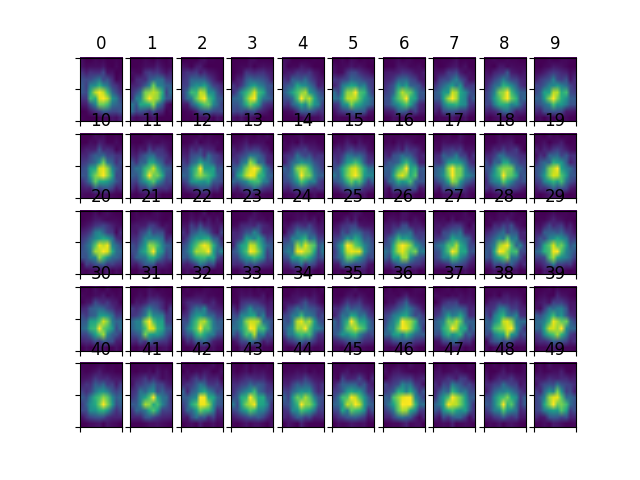
\includegraphics[scale=1]{visu_feature.png}

\end{figure}

\newpage
\begin{figure}
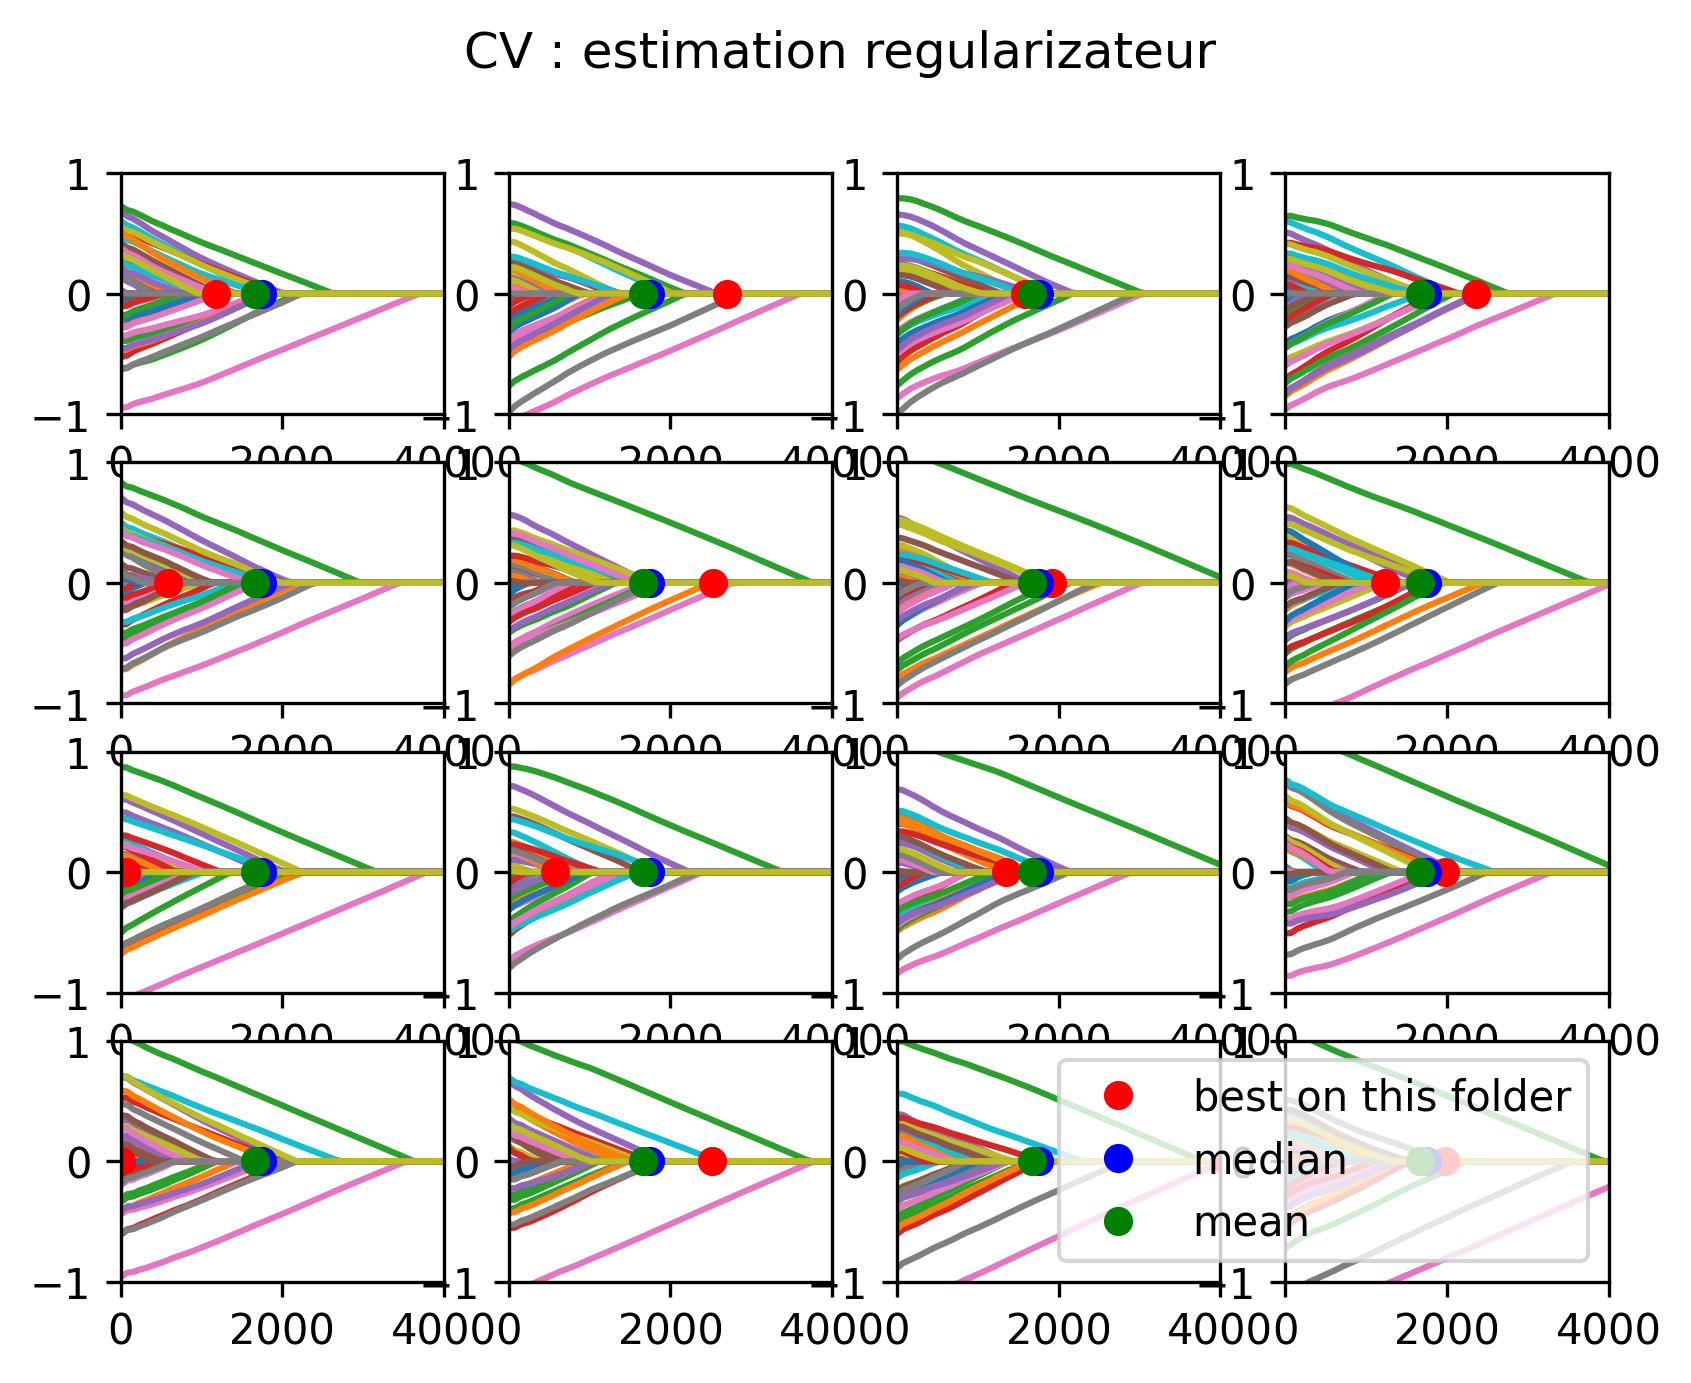
\includegraphics[scale=1]{cv_reg.png}

\end{figure}

\newpage
\newpage
\begin{figure}
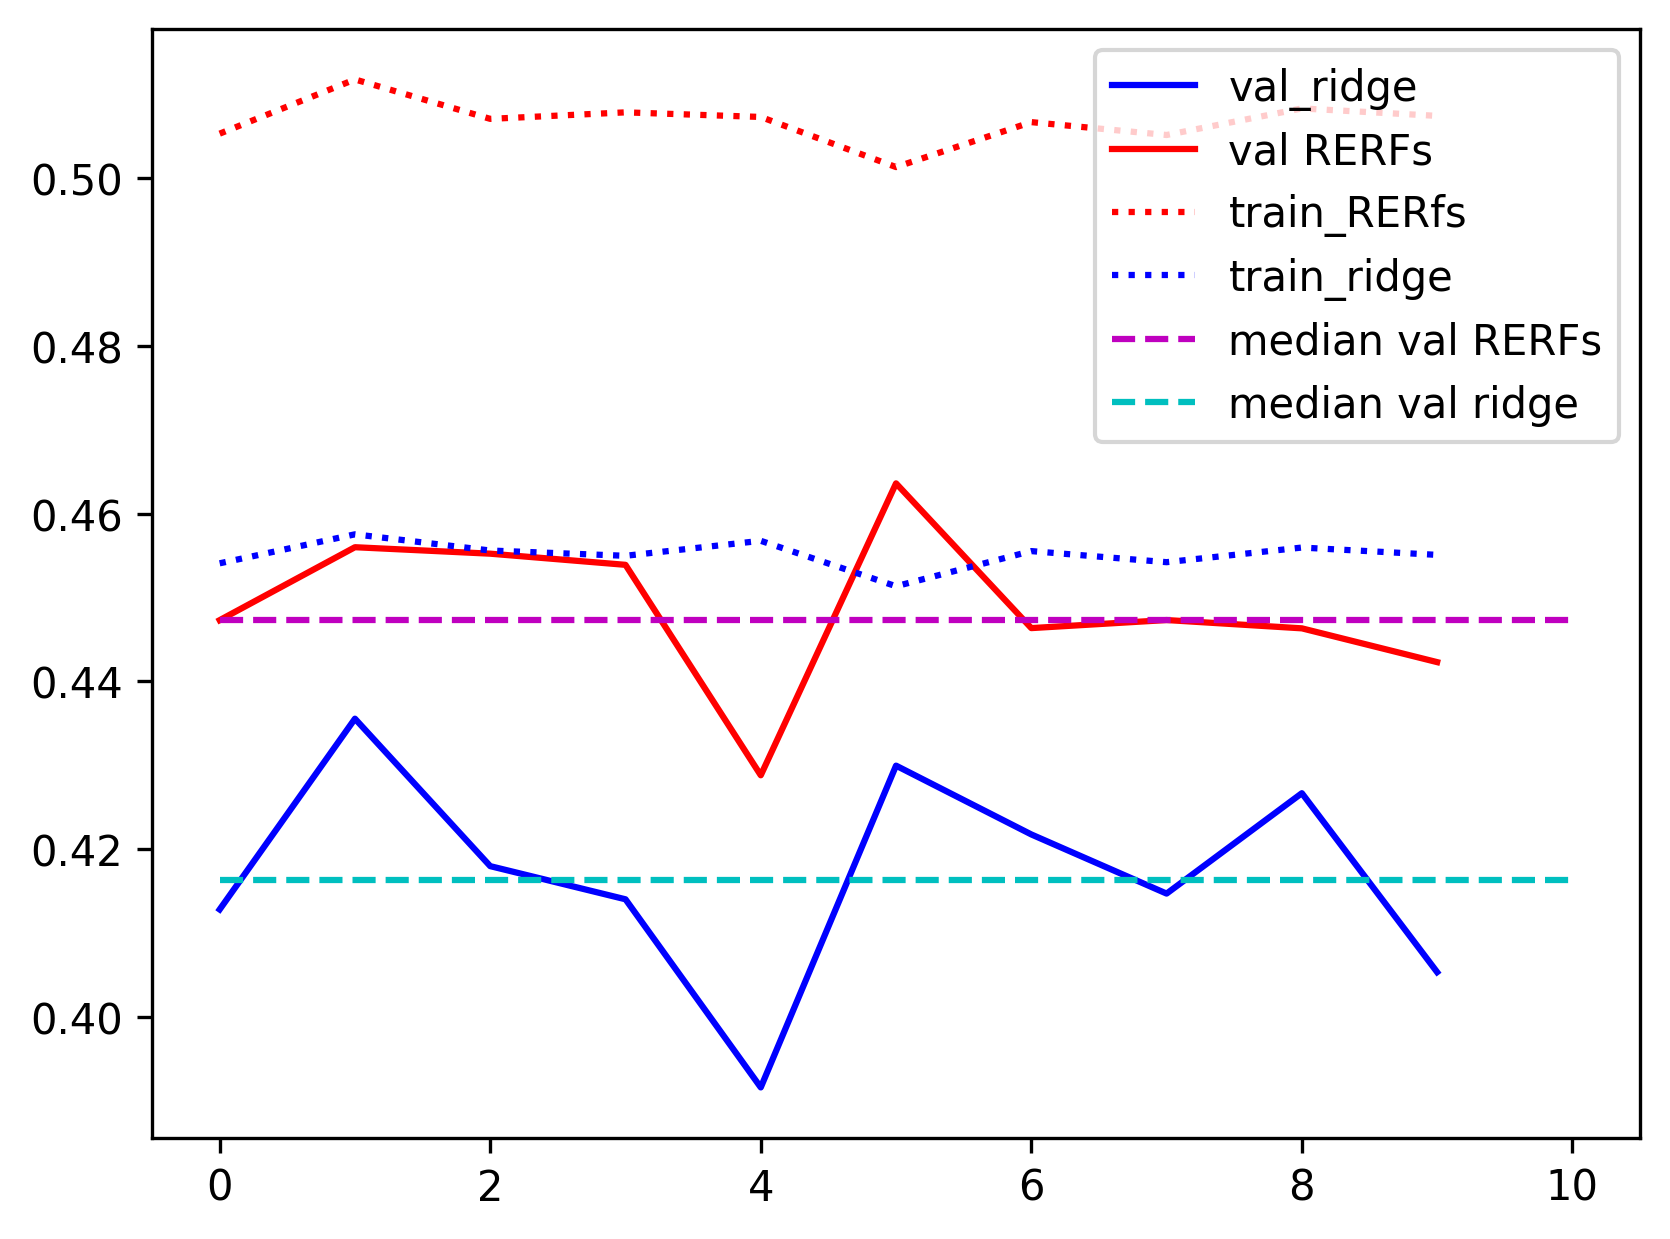
\includegraphics[scale=1]{compare.png}

\end{figure}


\newpage
\begin{figure}
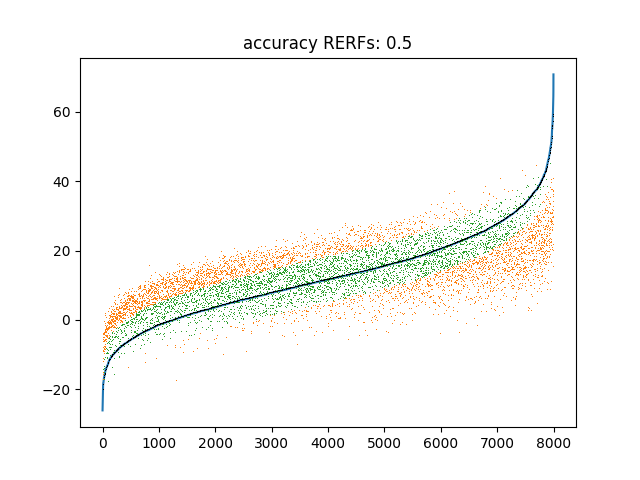
\includegraphics[scale=0.5]{pred_RERFsvs_true.png}
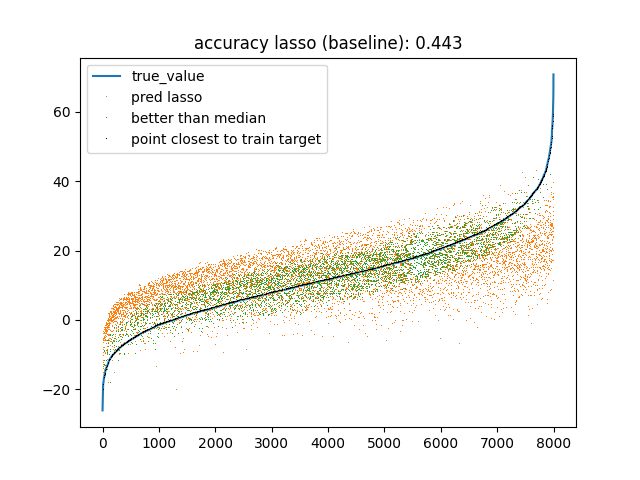
\includegraphics[scale=0.5]{pred_lasso_vs_true.png}
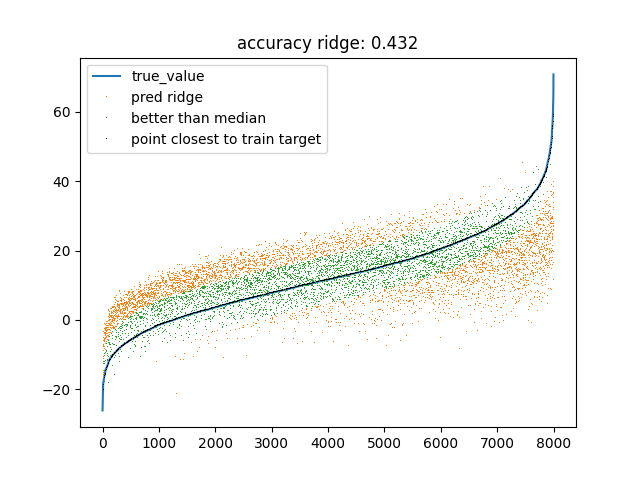
\includegraphics[scale=0.5]{pred_ridge_vs_true.png}
\end{figure}

\newpage

\begin{figure}
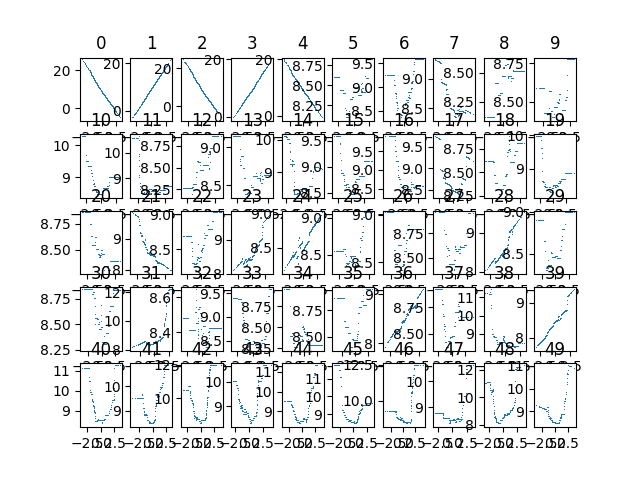
\includegraphics[scale=1]{affichage_fonction.png}
\end{figure}

\newpage

\begin{figure}
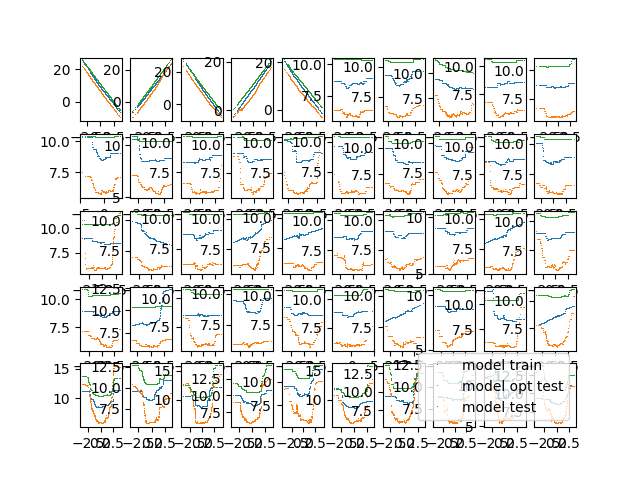
\includegraphics[scale=1]{affichage_fonction_test.png}
\end{figure}

\newpage

\begin{figure}
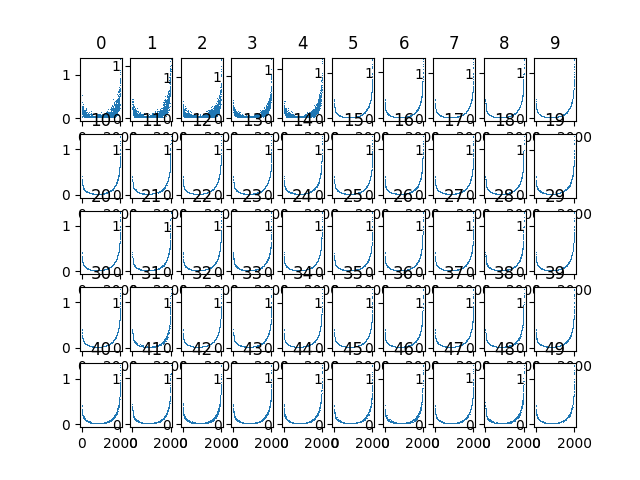
\includegraphics[scale=1]{error_par_feature.png}
\end{figure}

\newpage

\begin{figure}
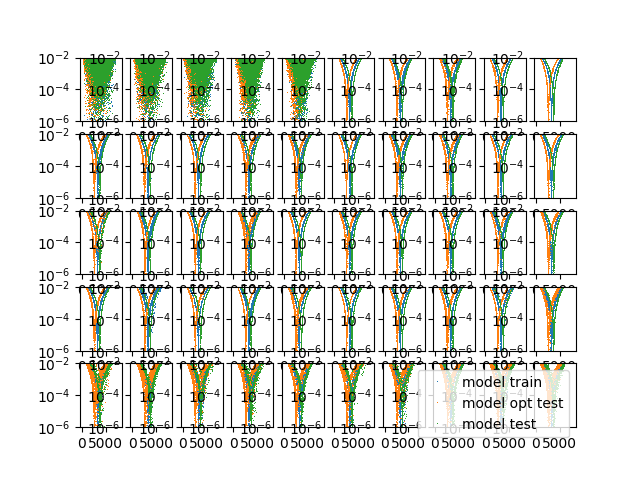
\includegraphics[scale=1]{error_par_feature_test.png}
\end{figure}

\newpage

\begin{figure}
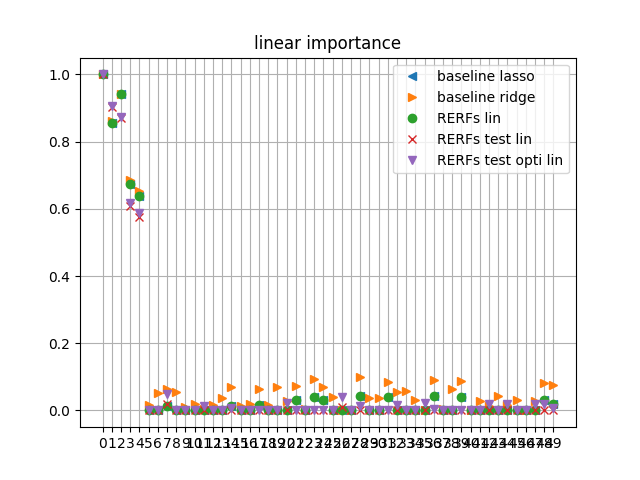
\includegraphics[scale=0.7]{linear_feature_importance.png}

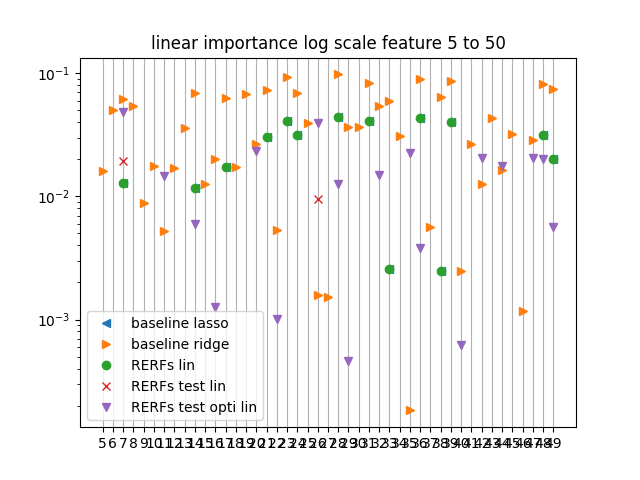
\includegraphics[scale=0.7]{linear_feature_importance2.png}

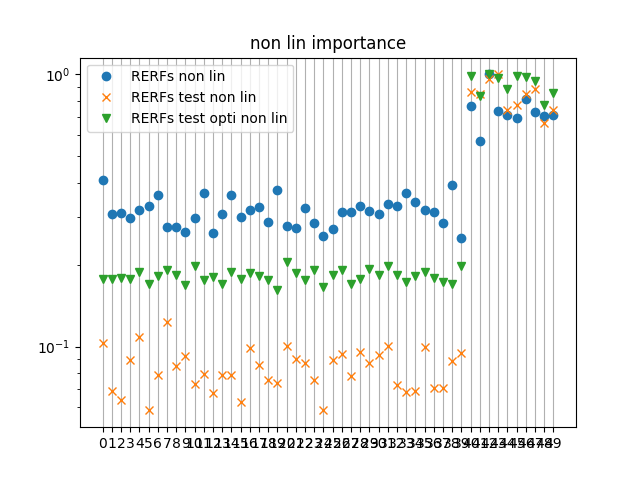
\includegraphics[scale=0.7]{non_linear_feature_importance.png}
\end{figure}
\end{document}

